\section{Materials and Methods}
The Armadillo IV will be driven a distance of 10 m several times. Each run will have a different setup for simulating different scenarios. The power consumption will be measured during each run.  

\subsection{Materials}\label{Materials}
\begin{itemize}
	\item Armadillo IV with Vibro crop implement
	\item Turnigy 130A Watt Meter and Power Analyzer
	\item camera
\end{itemize}
The test aims to provide an estimate of the power consumption during normal use. The depth of the cultvator is adjusted to 1.5 cm relative to the front wheels, see figure \ref{fig:vibro_crop_working_depth}
\begin{figure}[hbtp]
	\centering
	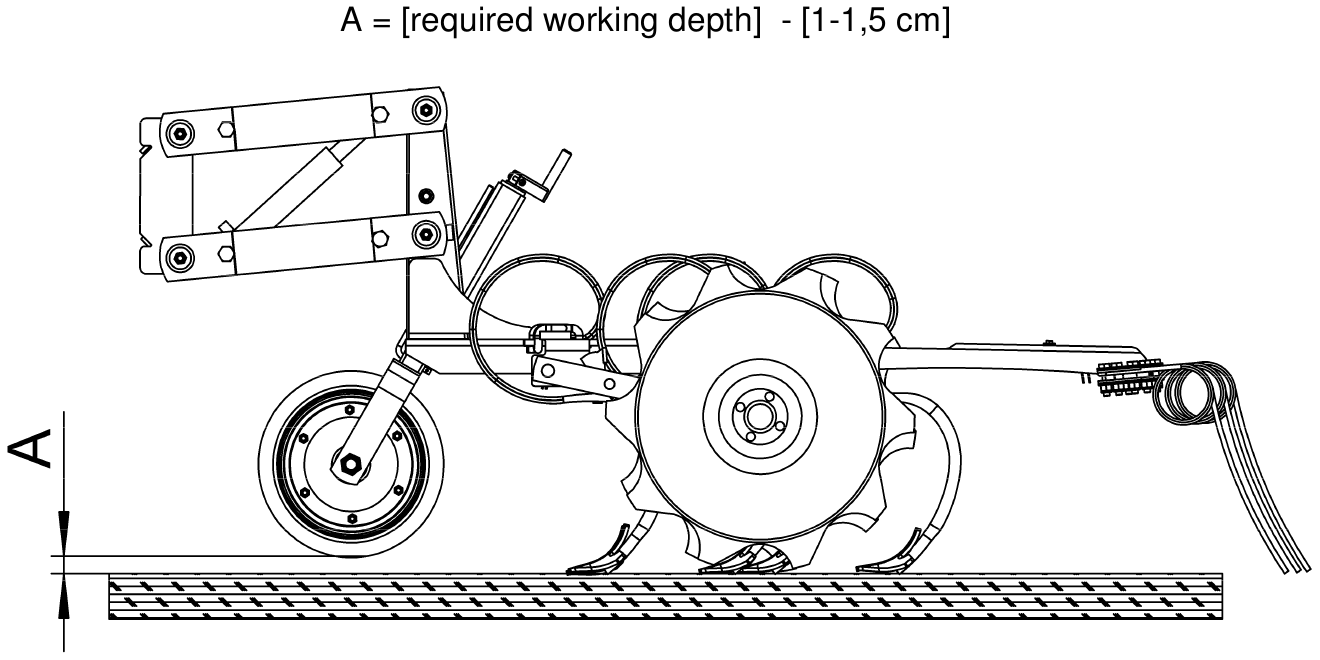
\includegraphics[width=0.7\linewidth]{./images/vibro_crop_working_depth}
	\caption{Working depth of cultivator during normal use}
	\label{fig:vibro_crop_working_depth}
\end{figure}
 
The test will be conducted on a piece of field that hasn't previously be been processed. Driving on previously processed land would provide soil that is easier to drag the cultivator through and thereby produce a lower power consumption than on unprocessed land. 

The motor controllers include a way for measuring of the power consumption. This data can be accessed through ROS bag. The tests will also be used to see in the internal power measuring will produce results similar to the Turnigy wattmeter.
Stikword:

	- Hvordan vurdere vi troværdigheden af data/dataanalyse
